 \documentclass[11pt,fleqn,a3]{article}
\usepackage{graphicx} %%%%%%%%%%%%%%% for inserting EPS pictures
\usepackage{amsmath}% AMS math equation
\usepackage{txfonts}
\usepackage{bm}
\usepackage{float}
\usepackage{tikz}
\usepackage{pgfplots}
\usepackage{longtable}
%
%**************************************************************%
%                   File Name: deffile.tex                     %
%                                                              %
%  This LaTeX file is prepared for writing the manuscript for  %
%    the 12th International Offshore and Polar Engineering     %
%   Conference to be held from May 26-31, 2002 in Kitakyushu   %
%      Organized by ISOPE and hosted by Kyushu University      %
%                                                              %
%           Prepared by Masashi KASHIWAGI on December 13, 2001 %
%**************************************************************%
%
\makeatletter
%%%%%%%%%%%%%%%%%%%%%%% Style of Footer %%%%%%%%%%%%%%%%%%%%%%%%%%%%%%
\def\ps@isopefoot{\let\@mkboth=\@gobbletwo
 \def\@oddhead{}
 \def\@evenhead{}
%\def\@oddfoot{}
%\def\@evenfoot{}
 \def\@oddfoot{\hbox to \textwidth
   {\footnotesize {Paper No.\,2011-\papernumber} \hfil 
   {\firstauthorname} \hfil {Page number:\ \thepage\ of\ \totalpage}}}
 \def\@evenfoot{\hbox to \textwidth
   {\footnotesize {Paper No.\,2011-\papernumber} \hfil 
   {\firstauthorname} \hfil {Page number:\ \thepage\ of\ \totalpage}}}
}%
%---------------------------------------------------------------
\setcounter{topnumber}{3}     %
\def\topfraction{1.0}         %
\setcounter{bottomnumber}{2}  %
\def\bottomfraction{1.0}      %
\setcounter{totalnumber}{4}   %
\def\textfraction{0.0}        %
\def\floatpagefraction{1.0}   %
%
\setcounter{dbltopnumber}{4}
\def\dbltopfraction{1.0}
\def\dblfloatpagefraction{1.0}
%---------------------------------------------------------------
%
\def\leftcapmargin{35pt}
\def\rightcapmargin{15pt}
%
\long\def\@makecaption#1#2{%
 \vskip 10\p@ \footnotesize\baselineskip=4.0mm
 \@tempdimb=\leftcapmargin
 \@tempdima\hsize\advance\@tempdima-\@tempdimb
 \@tempdimb=\rightcapmargin
 \advance\@tempdima-\@tempdimb
 \newbox\tempbox
 \setbox\tempbox=\hbox{#1}
 \setbox\@tempboxa=\hbox{\hskip\leftcapmargin #2\hskip\rightcapmargin}
 \ifdim \wd\@tempboxa >\hsize
 \hbox to\hsize{\hfil \hskip-\the\wd\tempbox \hskip\leftcapmargin #1 
 \parbox[t]\@tempdima{#2}\hskip\rightcapmargin}%
 \else \hbox to\hsize{\hfil #1 #2\hfil}\fi
%\setcounter{subfigure}{0}
%\setcounter{subtable}{0}
}
%--------------------------------------------------------
\def\fnum@figure{{\footnotesize Fig.\,\thefigure}\ }
\def\fnum@table{{\footnotesize Table\,\thetable}\,}
%
%%%%%%%%%%%%%%%%%%%%%%%%%%%%%%%%%%%%%%%%%%%%%%%%%%%%%%%%%%%%%%%%%%%%%%
\def\thesection{}
\def\thesubsection{}
\def\thesubsubsection{}
%
\def\section{\@startsection{section}{1}{\z@}
{2ex plus .3ex minus .2ex}{1.5ex plus .1ex}{\small}}
\def\subsection{\@startsection{subsection}{2}{\z@}
{1.5ex plus .2ex minus .2ex}{1ex plus .1ex}{\small\bf}}
\def\subsubsection{\@startsection{subsubsection}{3}{\z@}
{1.5ex plus .2ex minus .2ex}{1ex plus .1ex}{\footnotesize\it}}
%
\def\paragraph{\@startsection{paragraph}{4}{\z@}
{1ex plus .3ex minus .2ex}{-1em}{\large\bf}}
\def\subparagraph{\@startsection{subparagraph}{4}
{\parindent}{1ex plus .3ex minus .2ex}{-1em}{\small\bf}}
%---------------------------------------------------------------------
\def\eqnarray{%
 \stepcounter{equation}%
 \let\@currentlabel=\theequation
 \global\@eqnswtrue
 \global\@eqcnt\z@
 \tabskip\mathindent
 \let\\=\@eqncr
 $$\halign to \displaywidth\bgroup\@eqnsel\hskip\@centering
 $\displaystyle\tabskip\z@{##}$&\global\@eqcnt\@ne
 \hfil$\displaystyle{{}##{}}$\hfil
 &\global\@eqcnt\tw@$\displaystyle\tabskip\z@{##}$\hfil
 \tabskip\@centering&\llap{##}\tabskip\z@\cr}
%
%%%%%%%%%%%%%%%%%%%%%%%%%%%%%%%%%%%%%%%%%%%%%%%%%%%%%%%%%%%%%%%%%%%%%%
%
\def\@cite#1#2{\,[{\hbox{#1\if@tempswa , #2\fi}}]}
%
\def\thebibliography#1{%
\begin{flushleft}\section*{REFERENCES}\end{flushleft}
\list
{[\arabic{enumi}]}{\settowidth\labelwidth{#1)}\leftmargin\labelwidth
 \advance\leftmargin\labelsep
 \usecounter{enumi}}
 \def\newblock{\hskip .11em plus .33em minus .07em}
 \sloppy
 \sfcode`\.=1000\relax}
\let\endthebibliography=\endlist
%=====================================================================
%
\newif\if@lastpagecolumnalign \@lastpagecolumnaligntrue
% \@lastpagecolumnalignfalse  % if you do NOT need the function No.3
%
\if@lastpagecolumnalign %============ FUNCTION No.3 ============
%
\newdimen\lastp@geheight \lastp@geheight=10mm
\newsavebox{\lastp@gebox}
%
% define \endabstract
%
\long\def\endabstract#1{\gdef\@endabstract{#1}} % permit paragraphs
%
% to create enough space of footnote to align columns of the last page
%
\def\lastpagecontrol{\@ifnextchar [{\l@stpagecontrol}%
 {\l@stpagecontrol[\z@]}}
%
\def\l@stpagecontrol[#1]#2{\global\lastp@geheight=#2%
%
 \@ifundefined{maxsize}{}{\global\advance\maxsize-#2}% for supertab.sty
%
 \@ifundefined{@endabstract}{}{% save \endabstract in a box
 \global\sbox{\lastp@gebox}{%
  \begin{minipage}{\textwidth}\vspace*{#1}%
  \hrule width \textwidth \vspace{1ex}%
  \begin{list}{}{\setlength{\leftmargin}{0.15\textwidth}%
  \listparindent=10pt \parsep=0pt
  \topsep=0pt \partopsep=0pt
  \setlength{\rightmargin}{\leftmargin}\small}%
  \item \ignorespaces\hspace*{\listparindent}\ignorespaces
                 \@endabstract
  \end{list}%
  \vspace{1ex} \hrule width \textwidth
  \end{minipage}}}%
%
% insert footnote with abstract if enough room left
%                 without abstract otherwise
%
  \@tempdima\ht\lastp@gebox \advance\@tempdima\dp\lastp@gebox
 \ifdim\@tempdima>\lastp@geheight
  \@tempdima\lastp@geheight \global\lastp@geheight=0pt
 \else
  \global\advance\lastp@geheight -\@tempdima
  \@tempdima\lastp@geheight \global\lastp@geheight\textheight
 \fi
  \def\footnoterule{\null}% force it to \null at the last page
  \insert\footins{\footnotesize
  \interlinepenalty\interfootnotelinepenalty
  \splittopskip\footnotesep
  \splitmaxdepth \dp\strutbox \floatingpenalty \@MM
  \hsize\textwidth \@parboxrestore
  \ifdim\lastp@geheight=\z@\else\usebox{\lastp@gebox}\fi%
  \vspace*{\@tempdima}}}
%
% set the layout of the last line of the document
%
\def\lastpagesettings{\@ifnextchar [{\l@stpagesettings}%
 {\l@stpagesettings[\z@]}}
%
\def\l@stpagesettings[#1]{%
%\begin{flushright}%
% {\footnotesize(`{\tt\jobname.tex}'~~@~\today)}%
%\end{flushright}%
%
% put \endabstract in the next page when no room left for it
%
 \ifdim\lastp@geheight=\z@
 \onecolumn\null\vspace*{#1}\noindent\usebox{\lastp@gebox}%
 \fi}
%
\fi %===========================================================
%
\makeatother
%---------------------------------------------------------------
\def\jsection#1{\section{\hspace*{-4.0mm}\uppercase{#1}}}
\def\jsubsection#1{\subsection{\hspace*{-4.0mm}#1}}
\def\jsubsubsection#1{\subsubsection{\hspace*{-4.0mm}#1}}
%---------------------------------------------------------------
%%%%%%%%%%%%%%%%%%%%%%%%%%%%%%%%%%%%%%%%%%%%%%%%%%%%%%%%%%%%%%%%
\autospacing
\newcommand{\bdm}{\begin{displaymath}}
\newcommand{\edm}{\end{displaymath}}
\newcommand{\be}{\begin{equation}}
\newcommand{\ee}{\end{equation}}
\newcommand{\bea}{\begin{eqnarray}}
\newcommand{\eea}{\end{eqnarray}}
% 
\newcommand{\bc}{\begin{center}}
\newcommand{\ec}{\end{center}}
\newcommand{\bfl}{\begin{flushleft}}
\newcommand{\efl}{\end{flushleft}}
\newcommand{\bfr}{\begin{flushright}}
\newcommand{\efr}{\end{flushright}}
\newcommand{\ds}{\displaystyle}
%---------------------------------------------------------------
\newcommand{\mbf}[1]{\mbox{\boldmath$#1$}}
\newcommand{\ubar}[1]{\overline{#1}}
\newcommand{\dint}{\int\!\!\!\int}
\newcommand{\tint}{\int\!\!\!\int\!\!\!\int}
\newcommand{\heikou}{\,/\!/\,}
\newcommand{\hs}{\hspace*{0.2mm}}
\newcommand{\iomega}{i\hspace*{0.25mm}\omega\hspace*{0.2mm}}
\newcommand{\jneqi}{j = \hspace*{-1.6mm}/\hspace*{0.5mm} i}
\newcommand{\rmP}{{\rm P}}
\newcommand{\rmQ}{{\rm Q}}
\newcommand{\cint}{\int_0^\infty \hspace*{-6.2mm}C\hspace*{3.8mm}}
\newcommand{\e}{\,e}
\newcommand{\noteq}{=\hspace*{-3.0mm}/\hspace*{1.25mm}}
\newcommand{\ch}{\hspace*{0.5mm}{\rm ch}\hspace*{0.3mm}}
\newcommand{\sh}{\hspace*{0.5mm}{\rm sh}\hspace*{0.3mm}}
\newcommand{\dash}{{\hs\prime}}
\newcommand{\npar}{\par\vspace*{10pt}}
%
%%%%%%%%%%%%%%%% Upper case of Greek Letters %%%%%%%%%%%%%%%%%%
\newcommand{\gPi}{\mathnormal{\Pi}}
\newcommand{\gGamma}{\mathnormal{\Gamma}}
\newcommand{\gPhi}{\mathnormal{\Phi}}
\newcommand{\gPsi}{\mathnormal{\Psi}}
\newcommand{\gTheta}{\mathnormal{\Theta}}
\newcommand{\gDelta}{\mathnormal{\Delta}}
\newcommand{\gXi}{\mathnormal{\Xi}}
\newcommand{\gLambda}{\mathnormal{\Lambda}}
\newcommand{\gOmega}{\mathnormal{\Omega}}
%
%%%%%%%%%%%%%%%%%%%%%%%%%%%%%%%%%%%%%%%%%%%%%%%%%%%%%%%%%%%%%%%
\setlength{\textheight}  {240.0mm}
\setlength{\textwidth}   {191.9mm}
\setlength{\columnsep}   {8.9mm}
\setlength{\parindent}   {0.0mm}
\setlength{\mathindent}  {0.0mm}
%
\newlength{\mybaselineskip}
\setlength{\mybaselineskip}{11pt}
\newlength{\myleftmargin}
\newlength{\mytopmargin} 
\setlength{\myleftmargin}  {11.0mm}
\setlength{\mytopmargin}   {13.0mm}
%%%%%% For the letter size (ISOPE Format) %%%%%%%%%%%%%
\setlength{\myleftmargin}  {12.0mm}
\setlength{\mytopmargin}   { 3.0mm}
%%%%%%%%%%%%%%%%%%%%%%%%%%%%%%%%%%%%%%%%%%%%%%%%%%%%%%%
\setlength{\oddsidemargin} {-1in}
\setlength{\topmargin}     {-1in}
\addtolength{\oddsidemargin}{\myleftmargin}
\addtolength{\topmargin}    {\mytopmargin}
\setlength{\headheight}  { 0.0mm}
\setlength{\footskip}    {20.0mm}
%
\sloppy


\pagestyle{empty}
%\pagestyle{isopefoot} 
%

\newcommand{\papernumber} {TPC-970}
\newcommand{\firstauthorname} {Martin Alexandersson}
\newcommand{\totalpage} {10}
%
%+-+-+-+-+-+-+-+-+-+-+-+-+-+-+-+-+-+-+-+-+-+-+-+-+-+-+-+-+-+-+-+-+
\begin{document}
\baselineskip \mybaselineskip
\twocolumn[ 
    \par\vspace*{40.0mm}
    \large\bc{ \bf
        Prediction of ship roll decay motion using fully nonlinear potential flow and Ikeda’s method
    }\ec 

    \par\vspace{1mm}\footnotesize\bc
    {
        \small\it
        Martin Alexandersson
    }\\ 
    Department of Mechanics and Maritime Sciences, Chalmers University of Technology, Sweden \\
    SSPA Sweden AB, Gothenburg, Sweden\\
    {
        \small\it
        Martin Kjellberg
    }\\
    SSPA Sweden AB, Gothenburg, Sweden\\
    {
        \small\it
        Wengang Mao
    }\\
     Department of Mechanics and Maritime Sciences, Chalmers University of Technology, Sweden\\
    {
        \small\it
        Jonas W. Ringsberg
    }\\
     Department of Mechanics and Maritime Sciences, Chalmers University of Technology, Sweden\\

%
%%%%%%%%%%%%%%%%%%%%%%%%%%%%%%%%%%%%%%%%%%%%%%%%%%%%%%%%%%%%%%%%%%
\ec\par\vspace*{15mm}

]
\footnotesize\par\noindent{\small ABSTRACT}\par\vspace*{2.0mm}
\baselineskip \mybaselineskip

\section{Abstract}\label{abstract}

Many cost-efficient computational methods have been developed over the
years to analyze various aspects of ship hydrodynamics such as:
resistance, propulsion and seakeeping. Getting the best possible
accuracy with the lowest possible computational cost is an important
factor in a ship's early design stage. Potential flow-based analysis
partly presents such a solution for seakeeping, with good accuracy for
heave and pitch, but not for roll where the roll damping contains both
inviscid and viscous effects. Roll motion is, however, often a critical
degree of freedom that needs to be analyzed since large roll motions can
result in cargo shifting or even capsizing. The viscous part of roll
damping can be assessed with high accuracy by means of experimental
model tests or URANS calculations, but these are generally too expensive
in the early design stage of ships. Many semi-empirical formulas to
determine viscous damping were therefore developed during the 1970s,
where Ikeda's method is one of the most widely used. The viscous damping
from this method is normally combined with inviscid roll damping from
strip theory. With today's computational power, more advanced potential
flow methods can be used in the seakeeping analysis to enhance the
accuracy in the predictions, but still at relatively low computational
cost. This paper investigates the feasibility of combining 3D unsteady
fully nonlinear potential flow (FNPF) theory solved by means of a
Boundary Element Method (BEM) together with the viscous contributions
from Ikeda's method. The approach of substituting the inviscid part from
Ikeda's method using strip theory with FNPF is investigated by
conducting roll decay simulations. The results estimated by the proposed
approach are compared with both the classical strip theory approach and
roll decay model tests. It is found that potential improvements to the
modelling of roll damping can be achieved by introducing FNPF analysis
in Ikeda's method.

    
%-----------------------------------------------------------------
\footnotesize
\par\bigskip\noindent{{\small KEY\,\,WORDS}}:
%%%%%%%%%%%%%%%%%%%%%%%%%%%%%%%%%%%%%%%%%%%%%%%%%%%%%%%%%%%%%%%%%%
%%%%%%%%%%%%%%%%%%%%%%% Write Key Words %%%%%%%%%%%%%%%%%%%%%%%%%%
%%%%%%%%%%%%%%%%%%%%%%%%%%%%%%%%%%%%%%%%%%%%%%%%%%%%%%%%%%%%%%%%%%
Roll-decay; Roll-damping; Ikeda's method; Fully nonlinear potential flow (FNPF); Boundary element methods.
%
\par\vspace*{2mm}%
%%%%%%%%%%%%%%%%%%%%%%%%%%%%%%%%%%%%%%%%%%%%%%%%%%%%%%%%%%%%%%%%%%
%%%%%%%%%%%%%%%%%%%%%%% Start Introduction %%%%%%%%%%%%%%%%%%%%%%%
%%%%%% Please use \jsection{ .... } or \section*{ ..... } %%%%%%%%
%%%%%%%%%%%%%%%%%%%%%%%%%%%%%%%%%%%%%%%%%%%%%%%%%%%%%%%%%%%%%%%%%%
%\jsection{Introduction}
%%-----------------------------------------------------------------
%\section*{INTRODUCTION}\label{introduction}
Inviscid potential flow calculations can be used to solve seakeeping
problems at very low computational costs. These methods offer far
cheaper alternatives than doing for instance model tests or URANS
calculations. Potential flow calculations can therefore be used
extensively during the early design stage of ships. The pitch and heave
motions can be predicted with good accuracy, even with the older linear
strip theory methods \citep{7505983/FB64RGPF}. The roll motions will
however not be very realistic in potential flow, due to high influenced
from viscous roll damping. This is very unfortunate as the roll motions
is indeed a very important response. The impact of roll motions can be
seen from the APL China casualty in 1998, where a post-Panamax C11 class
container ship lost almost a third of its containers
\citep{7505983/WPADAQB3}. Another example is the container ship Svendborg
Maersk, were 500 containers were lost overboard and 250 containers were
damaged as a result of heavy roll motions during a passage from English
Channel to Gibraltar \citep{7505983/T78CMTDR}.
\quad A lot of experimental research was conducted during the 1970s and
80s to separate the invicid and viscous roll damping. Semi empirical
formulas were developed to estimate the viscous parts, to be used
together with the potential flow methods \citep{7505983/937PN5DT}. The
older linear methods can today be replaced by more advanced nonlinear
potential flow methods. These newer methods still need some injection of
semi empirical viscous damping to give a fair representation of the roll
motions. But is the separation of damping components still valid,
considering that these older semi empirical methods were developed in
close connection to linear strip theory? \citep{7505983/UGK6YEVD} have
shown that the separation of viscous and invicid damping is still valid
for a panel method and Ikeda's method to predict the roll motion for the
mentioned APL China vessel. \citep{7505983/24TNAV5Z} have investigated an
even more advanced method, using a fully nonlinear potential flow method
(FNPF) \citep{7505983/P4XDUMMQ} combined with Watanabe and Inoue method
(W-I) \citep{7505983/ARMIRMVY} to predict the viscous damping for the DTC
test case \citep{7505983/BYNJ8CFG}. This FNPF method is used also in the
present paper, but instead of W-I method, Ikeda's method is instead
used. Ikeda's method is believed to be a good method for the purpose,
based on results from a previous comparisons of a large number of model
scale roll decay tests \citep{7505983/QMGQ76Q9}.
\quad The implementation of the proposed hybrid method is introduced in
the next section where the underlying Ikeda's method and FNPF method are
both presented. The implementation of Ikeda's method is also closely
examined and an alternative way to calculate eddy damping is proposed.
In the validation study of the hybrid method, roll decay tests from
model tests are compared with simulations for the KVLCC2 test case. In
the roll decay tests, both decay and frequency can be observed, without
the presence of external forces from wind and waves. This gives a good
indication of the ship's roll damping and inertia. A more thorough
description of the roll decay test is given in the Roll decay test
section of this paper.

%
%\medskip%%%%%%%%%%%%%%%%%%%%%%%%%%%%%%%%%%%%%%%%%%%%%%%%%%%%%%%%%%%%%%
%%%%%%%%%%%%%%%%%%%%%%%%%%%% Next Section %%%%%%%%%%%%%%%%%%%%%%%%%%%%%
%%%%%%%%% Please use \jsection{ .... } or \section*{ ..... } %%%%%%%%%%
%%%%%%%%%%%%%%%%%%%%%%%%%%%%%%%%%%%%%%%%%%%%%%%%%%%%%%%%%%%%%%%%%%%%%%%

%\section*{NOMENCLATURE}\label{nomenclature}
\vspace{-1.3cm}
\mbox{}
\nomenclature{$\displaystyle AP$,$\displaystyle FP$}{ship perpendiculars\nomunit{-}}
\nomenclature{$\displaystyle A_{44}$}{total mass moment of inertia\nomunit{kg*m^2}}
\nomenclature{$\displaystyle B'_{E0}$}{zero speed sectional eddy damping\nomunit{Nm*s/(m)}}
\nomenclature{$\displaystyle B_{1}$,$\displaystyle B_{2}$,$\displaystyle B_{3}$,$\displaystyle C_{1}$,$\displaystyle C_{3}$,$\displaystyle C_{5}$}{stiffness coefficient\nomunit{Nm}}
\nomenclature{$\displaystyle B_{1A}$,$\displaystyle B_{2A}$,$\displaystyle B_{3A}$}{damping helpers\nomunit{ }}
\nomenclature{$\displaystyle B_{E0}$}{zero speed eddy damping \nomunit{Nm*s}}
\nomenclature{$\displaystyle \hat{B}_{E0}$}{eddy roll damping at zero speed\nomunit{-}}
\nomenclature{$\displaystyle \hat{B^*}_{E}$}{only nonlinear nondimensional eddy damping\nomunit{-}}
\nomenclature{$\displaystyle \hat{B^*}_{F}$}{only nonlinear nondimensional friction damping\nomunit{-}}
\nomenclature{$\displaystyle \hat{B^*}_{W}$}{only nonlinear nondimensional wave damping\nomunit{-}}
\nomenclature{$\displaystyle B_{s}$}{section beam\nomunit{m}}
\nomenclature{$\displaystyle \hat{B^*}$}{only nonlinear nondimensional damping\nomunit{-}}
\nomenclature{$\displaystyle C_{1A}$,$\displaystyle C_{3A}$,$\displaystyle C_{5A}$}{stiffness helpers\nomunit{ }}
\nomenclature{$\displaystyle C_{r}$}{eddy damping coefficient\nomunit{-}}
\nomenclature{$\displaystyle D_{1}$,$\displaystyle a_{1}$,$\displaystyle a_{3}$}{lewis section coefficient\nomunit{-}}
\nomenclature{$\displaystyle H_{0}$}{half beam-draft ratio\nomunit{-}}
\nomenclature{$\displaystyle R_{b}$}{bilge radius\nomunit{m}}
\nomenclature{$\displaystyle T_{s}$}{section draught\nomunit{m}}
\nomenclature{$\displaystyle beam$}{ship beam\nomunit{m}}
\nomenclature{$\displaystyle \omega$}{angular velocity of external moment\nomunit{rad/s}}
\nomenclature{$\displaystyle \omega_{0}$}{natural angular velocity\nomunit{rad/s}}
\nomenclature{$\displaystyle \hat{\omega}$}{nondimensional roll frequency\nomunit{-}}
\nomenclature{$\displaystyle \phi_{a}$}{roll amplitude\nomunit{rad}}
\nomenclature{$\displaystyle \rho$}{water density\nomunit{kg/m^3}}
\nomenclature{$\displaystyle \sigma$}{section area coefficient\nomunit{-}}
\nomenclature{$\displaystyle t$}{time\nomunit{s}}
\nomenclature{$\displaystyle \zeta$}{damping coefficient\nomunit{-}}
\printnomenclature
% Add a bibliography block to the postdoc


\section*{INTRODUCTION}\label{introduction}
Inviscid potential flow calculations can be used to solve seakeeping
problems at very low computational costs. These methods offer far
cheaper alternatives than doing for instance model tests or URANS
calculations. Potential flow calculations can therefore be used
extensively during the early design stage of ships. The pitch and heave
motions can be predicted with good accuracy, even with the older linear
strip theory methods \citep{7505983/FB64RGPF}. The roll motions will
however not be very realistic in potential flow, due to high influenced
from viscous roll damping. This is very unfortunate as the roll motions
is indeed a very important response. The impact of roll motions can be
seen from the APL China casualty in 1998, where a post-Panamax C11 class
container ship lost almost a third of its containers
\citep{7505983/WPADAQB3}. Another example is the container ship Svendborg
Maersk, were 500 containers were lost overboard and 250 containers were
damaged as a result of heavy roll motions during a passage from English
Channel to Gibraltar \citep{7505983/T78CMTDR}.
\quad A lot of experimental research was conducted during the 1970s and
80s to separate the invicid and viscous roll damping. Semi empirical
formulas were developed to estimate the viscous parts, to be used
together with the potential flow methods \citep{7505983/937PN5DT}. The
older linear methods can today be replaced by more advanced nonlinear
potential flow methods. These newer methods still need some injection of
semi empirical viscous damping to give a fair representation of the roll
motions. But is the separation of damping components still valid,
considering that these older semi empirical methods were developed in
close connection to linear strip theory? \citep{7505983/UGK6YEVD} have
shown that the separation of viscous and invicid damping is still valid
for a panel method and Ikeda's method to predict the roll motion for the
mentioned APL China vessel. \citep{7505983/24TNAV5Z} have investigated an
even more advanced method, using a fully nonlinear potential flow method
(FNPF) \citep{7505983/P4XDUMMQ} combined with Watanabe and Inoue method
(W-I) \citep{7505983/ARMIRMVY} to predict the viscous damping for the DTC
test case \citep{7505983/BYNJ8CFG}. This FNPF method is used also in the
present paper, but instead of W-I method, Ikeda's method is instead
used. Ikeda's method is believed to be a good method for the purpose,
based on results from a previous comparisons of a large number of model
scale roll decay tests \citep{7505983/QMGQ76Q9}.
\quad The implementation of the proposed hybrid method is introduced in
the next section where the underlying Ikeda's method and FNPF method are
both presented. The implementation of Ikeda's method is also closely
examined and an alternative way to calculate eddy damping is proposed.
In the validation study of the hybrid method, roll decay tests from
model tests are compared with simulations for the KVLCC2 test case. In
the roll decay tests, both decay and frequency can be observed, without
the presence of external forces from wind and waves. This gives a good
indication of the ship's roll damping and inertia. A more thorough
description of the roll decay test is given in the Roll decay test
section of this paper.

\section*{PROPOSED HYBRID METHOD}\label{proposed-hybrid-method}
A hybrid method is proposed in this paper, where wave damping $B_W$
(including the speed dependent wave damping) obtained implicitly with
FNPF is used together with the viscous damping contributions from
Ikeda's method. The viscous damping is added to the FNPF simulations by
injecting the viscous parts of the linear and quadratic damping
coefficients (obtained with Ikeda's method) to the equation of motion.
Ikeda's method divides roll damping into five damping components so that
the total damping can be calculated as \citep{7505983/937PN5DT},
\begin{equation}
B = B_F + B_E + B_L + B_W + B_{BK}
\end{equation}
Where $B_F$ is the skin friction component, $B_E$ is the eddy
generation component, $B_L$ is hull lift component, $B_W$ is roll
wave generation component and $B_{BK}$ is the bilge keel component.
Ikeda's method propose semi empirical formulas for the viscous damping
components: $B_F$, $B_E$, $B_{BK}$ and $B_L$ so that viscous
damping can be obtained from,
\begin{equation}
\label{eq:viscous_damping}
B_{visc} = B_F + B_E + B_L
\end{equation}
\quad In order to reduce the number of uncertain parameters, the bilge
keel damping $B_{BK}$ has been exluded in
Eq.\ref{eq:viscous_damping}, thereby assuming that the ship does
not have any bilge keels.
\quad The skin friction damping $B_F$ is calculated using
\citep{7505983/CKCMI3N9} which is implementation according to the
description in \citep{7505983/UGK6YEVD}. The scale effects of roll
damping are considered to mainly be associated with the skin friction
component $B_F$ \citep{7505983/FB64RGPF}. This component constitute a
very small part of the total damping for the full scale ship, but a
substantial part for the model scale ship used in this study. This is
therefore the only component in Ikedas method that needs to be
recalculated when the scale changes.
\quad The hull lift damping $B_L$ is calculated according to
\citep{7505983/937PN5DT} and implemented as described in
\citep{7505983/UYUAYY7E} where the calculations have been improved with a
linear interpolation of the values for $\kappa$ from
\citep{7505983/937PN5DT}.
\quad Ikeda's method calculates the roll damping at a certain roll angle
frequency $\omega$ and roll angle amplitude $\phi_a$. A schematic
graph of how the parameters vary with speed and roll angle amplitude
$\phi_a$ is shown in Fig.\ref{fig:ikeda_generic}. In this
figure, roll amplitude is first varied at zero speed (left). The speed
is then varied at constant roll angle amplitude of 10 degrees (middle).
The amplitude is then gradually reduced at the highest speed down to
zero again (right).
\quad Assumming that the trends are correct in Ikeda's method it can be
noted from the amplitude variations at zero knots (left):
\begin{itemize}
\item $B_W$ does not change with amplitude, implying that they only contribute to the linear part ($B_1$) of the damping. (The $B_W$ was calculated with strip theory here)
\item $B_F$ has a small amplitude dependancy but the linear part is dominating.
\item $B_E$ has a large amplitude depandancy and only contributes to the quadratic damping ($B_2$)\citep{7505983/4AFVVGNT}.
\end{itemize}
\quad Looking at the speed variation (middle):
\begin{itemize}
\item At low speed $B_F$ and $B_E$ are the dominating components. (Note that this ship does not have bilge keels, as that would otherwise also be a large component).
\item At high speed the $B_E$ has almost disappeared and is replaced by the $B_L$ which is now the dominating component.
\item $B_F$ has a large contribution for all speeds (at model scale).
\end{itemize}
\quad Looking at the roll amplitude variation (right):
\begin{itemize}
\item (Please note that this x-axis is revered in this graph)
\item $B_L$ does not change with amplitude, implying that they only contribute to the linear part ($B_1$) of the damping.
\item $B_F$ has a small amplitude dependancy but the linear part is dominating.
\end{itemize}
\begin{figure}[H]
\begin{center}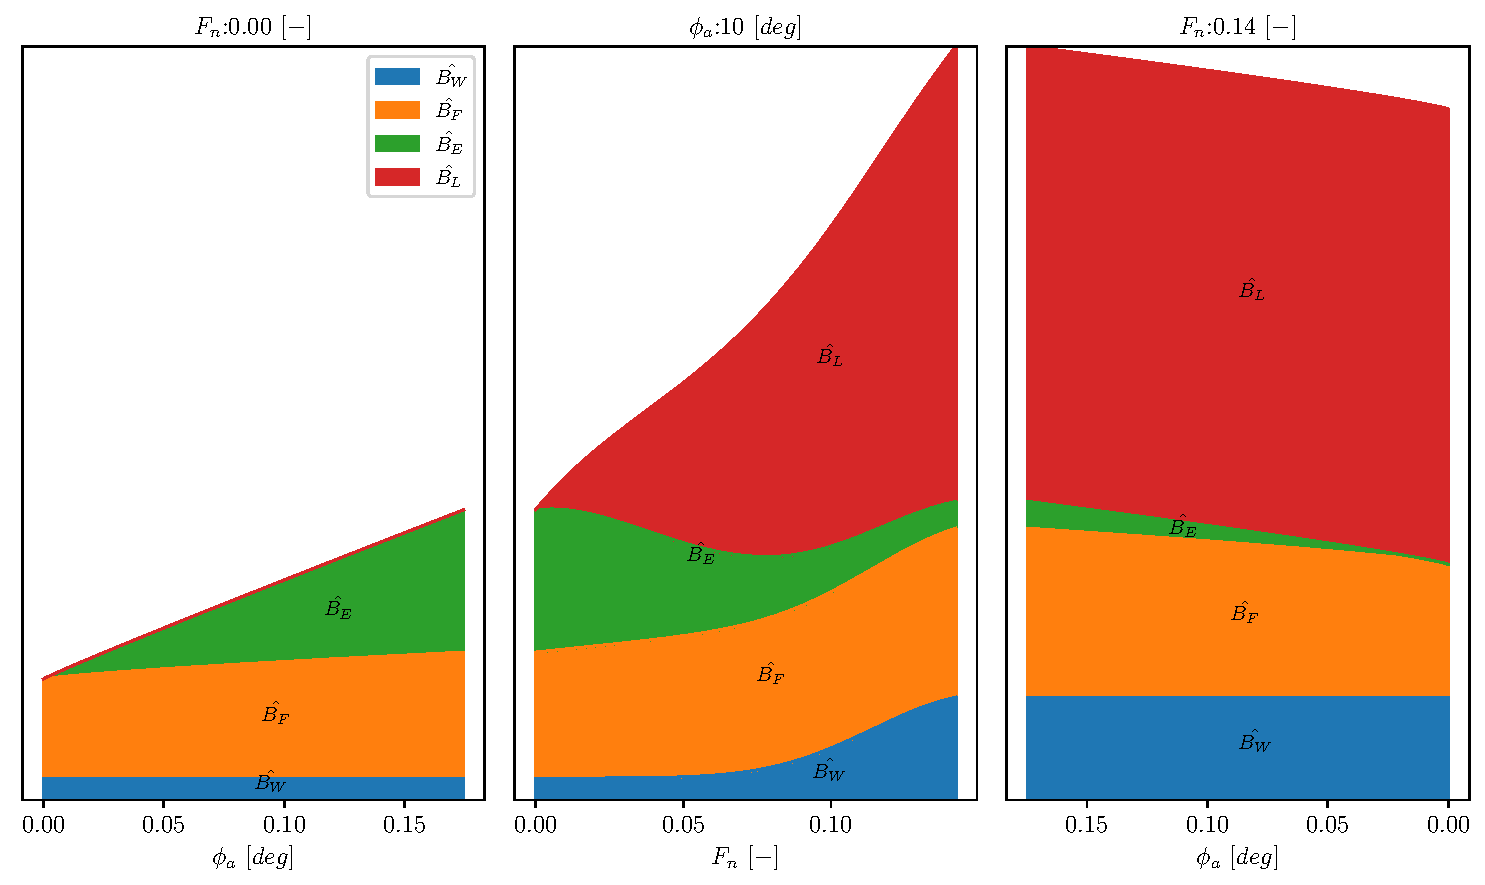
\includegraphics[width = 0.5\textwidth]{figures/ikeda_generic.pdf}\end{center}
\vspace{-1cm}
\caption{Example of roll damping predicted with Ikeda's method}
\label{fig:ikeda_generic}
\end{figure}
When the damping predicted with Ikeda's method was compared with
corresponding model tests (see section "\nameref{se:validation}"), it
was found that the results were in poor agreement for the zero speed
case (see Fig.\ref{fig:ikeda} (left)) but quite good results at
speed. This was pointing towards the eddy damping being incorrect in the
current implementation of Ikeda's method. A thorough investigation of
the eddy damping prediction was therefore conducted which is described
in the next section.
\subsection*{Eddy damping}\label{eddy-damping}
At zero speed, the eddy damping $B_E$ represents a nonlinear force
caused by the two-dimensional separation near the bilge keel. The eddy
damping is also nonlinear at speed where it represents the nonlinear
part part of the hydrodynamic lift damping ($B_L$ represents the
linear part). The speed dependancy of the eddy damping is calculated
using the following semi empirical formula \citep{7505983/937PN5DT}:
\begin{equation}
\frac{B_{E}}{B_{E0}} = \frac{0.0016 K^{2}}{0.0016 K^{2} + 1}
\label{eq:eddy_speed}
\end{equation}
Where $K$ is the reduced frequency:
\begin{equation}
K = \frac{L_{pp} \omega}{V}
\label{eq:K}
\end{equation}
For the zero speed case, Fig.\ref{fig:eddy_sigma} is an
illustration of how the eddy damping changes with bilge radius as
predicted with the current implementation of the method. It seems that
the damping approaches zero very fast as the bilge radius increases.
Having just a small rounding of the bilge, compared to a square section,
will thereby have a great impact on the eddy roll damping.
\begin{figure}[H]
\begin{center}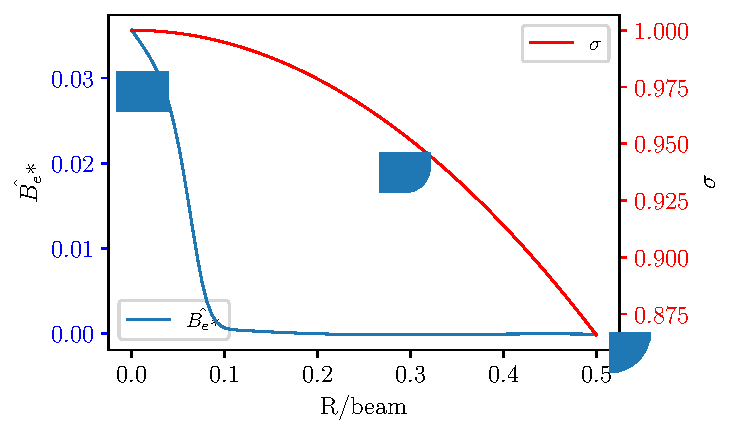
\includegraphics[width = 0.5\textwidth]{figures/eddy_sigma.pdf}\end{center}
\vspace{-1cm}
\caption{Sectional eddy damping (left y-axis) and $\sigma$ (right y-axis) vs. bilge radius (x-axis).}
\label{fig:eddy_sigma}
\end{figure}
The eddy damping prediction at zero speed is based on a regression
formula from experiements on a number of two-dimensional cylinders with
various sections \citep{7505983/4AFVVGNT}. The eddy damping per unit
length of these sections can be expressed as:
\begin{equation}
B'_{E0} = \frac{4 C_{r} T_{s}^{4} \omega \phi_{a} \rho}{3 \pi}
\label{eq:eddy_section}
\end{equation}
The total eddy damping can be obtained as an integral over the sections
along the ship hull:
\begin{equation}
B_{E0} = \int\limits_{AP}^{FP} B'_{E0}\, dx_{s}
\label{eq:eddy_integration}
\end{equation}
It can be seen from the section damping
(Eq.\ref{eq:eddy_section}) that the eddy damping increases
linearly with both roll amplitude and frequency, and that it will go to
zero for small amplitudes and frequencies. This means that eddy damping
is only included in the quadratic damping term ($B_2$). The $C_r$
coefficient in (Eq.\ref{eq:eddy_section}) is assumed to be
entirely depending on the hull form and is calculated using the
regression formula in \citep{7505983/4AFVVGNT}. This regression formula
is based on: section area coefficient $\sigma$ and the Lewis section
coefficients: $a_1$ and $a_3$. An alternative regression formula for
$C_r$ has however been developed for this paper, as described below.
This regression is based the same experimental results
\citep{7505983/4AFVVGNT}, collected by the authors using manual
digitalization \citep{7505983/8YUE24LM}.
The nondimensional damping taken from \citep{7505983/4AFVVGNT} is
expressed using an asterisk, or star symbol (*), to emphase that this
component only has a quadratic part of the damping. This stared damping
is defined as:
\begin{equation}
\hat{B}_{E0} = \frac{8 \hat{B^*}_{E}}{3 \pi}
\label{eq:B_E_star_hat}
\end{equation}
$\hat{B_E^*}$ and $(B_W+B_F)^*$ are the experimental values taken
from \citep{7505983/4AFVVGNT}. Which add up to the total damping:
\begin{equation}
\hat{B^*} = \hat{B^*}_{E} + \hat{B^*}_{F} + \hat{B^*}_{W}
\label{eq:B_star_hat}
\end{equation}
And the $C_r$ can be calculated from the experiments as:
\begin{equation}
C_{r} = \frac{3 \pi B_{s} \hat{B}_{E0} beam^{2} \sigma}{4 T_{s}^{3} \hat{\omega} \phi_{a}}
\label{eq:C_r_2}
\end{equation}
A simple decision tree model is used for the $C_r$ regression, based
on the same Lewis section coefficients from the regular regression
formula. The fitted decision tree is illustrated in
Fig.\ref{fig:decision_tree}.
\begin{figure}[H]
\begin{center}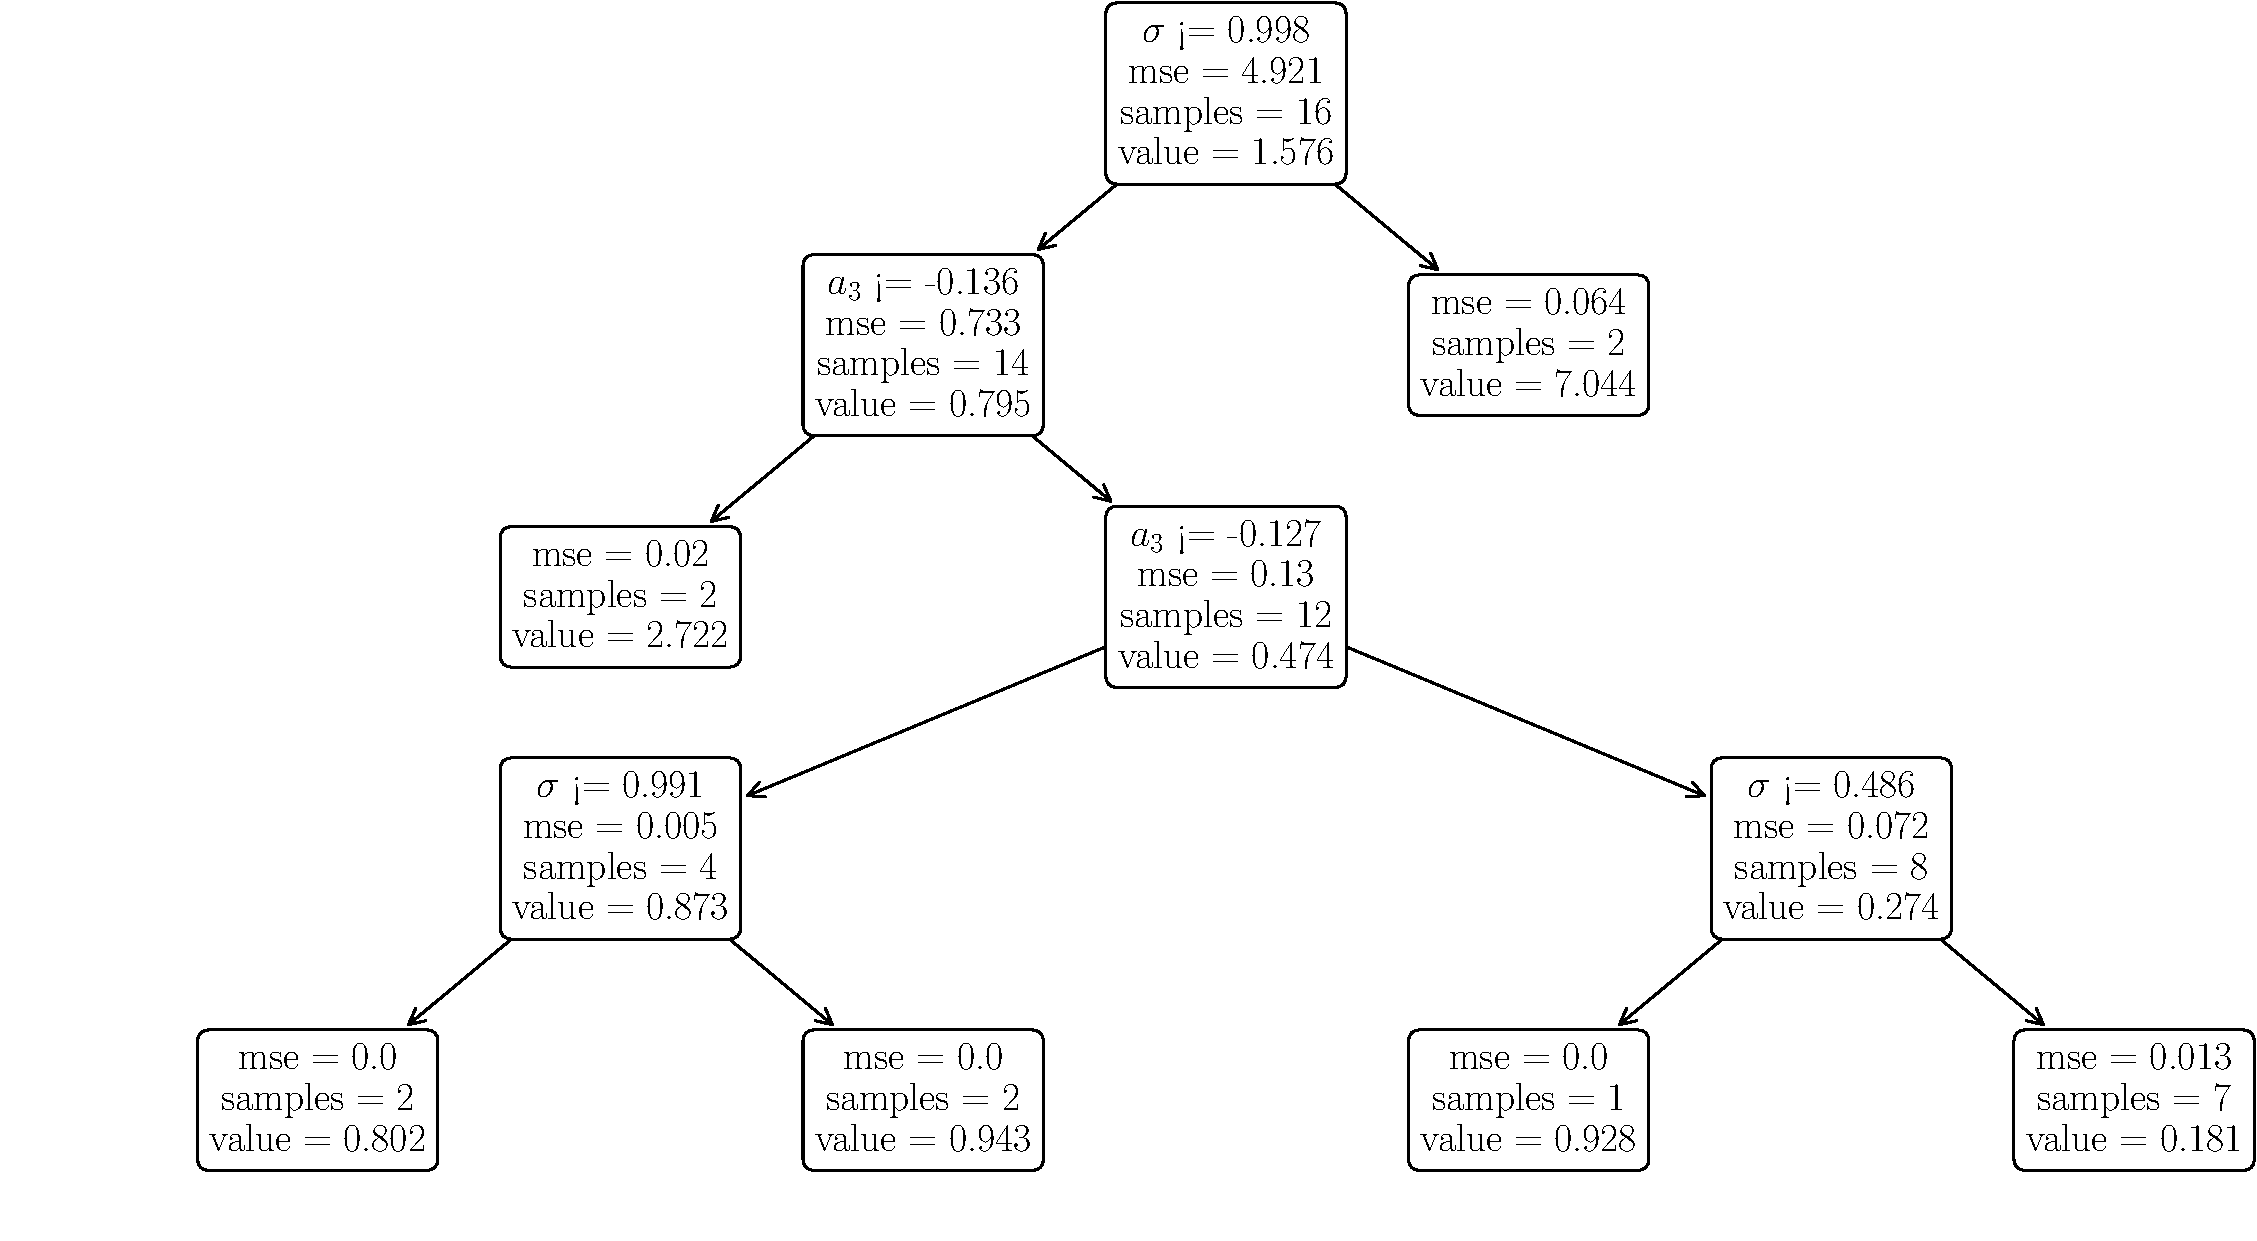
\includegraphics[width = 0.5\textwidth]{figures/decision_tree.pdf}\end{center}
\vspace{-1cm}
\caption{Decision tree to predict $C_r$}
\label{fig:decision_tree}
\end{figure}
Even though this tree is very simple it has very good accuracy in
reproducing the results from Ikedas experiments ($r^2=0.996$) compared
to ($r^2=0.762$) when using Ikeda's method.
Fig.\ref{fig:ikeda_sections} shows $C_r$ from the experiments
and corresponding predictions with Ikeda's method and the decision tree.
The capital letters refer to cylinder sections from the experiments
\citep{7505983/4AFVVGNT}.
\begin{figure}[H]
\begin{center}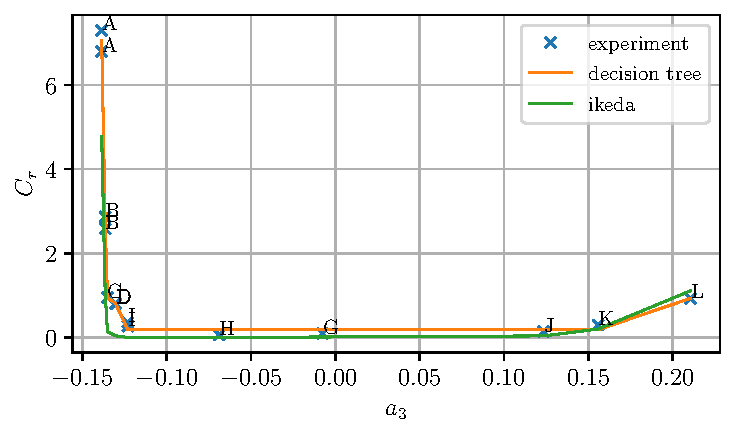
\includegraphics[width = 0.5\textwidth]{figures/ikeda_sections.pdf}\end{center}
\vspace{-1cm}
\caption{$C_r$ for cylinder sections from experiments and predicted with Ikeda's method and the decision tree model.}
\label{fig:ikeda_sections}
\end{figure}
\subsection*{FNPF method}\label{fnpf-method}
\label{fnpf-method} The wave damping was obtained using parameter an
identification technique, as described in section: "\nameref{se:pit}",
on roll decay simulation using the fully nonlinear potential flow
method. This method is characterized by the application of the complete
dynamic and kinematic free surface boundary conditions on the
instantaneous free surface as well as the body-exact approach where the
instantaneous wetted body surface is considered in the boundary value
problem for the velocity potential, i.e. no linearizations are made to
the governing equations of the potential flow problem.
\quad The method used in this study employs a boundary element method
(BEM) \citep{7505983/FD4N3DW2} to solve the boundary value problem for
the velocity potential.
\quad The free surface boundary conditions and the motions of the
floating body introduce time dependency to the boundary value problem.
The BEM is coupled with the mixed Eulerian-Lagrangian method (MEL)
\citep{7505983/ZKB494GT} which is used for the evolution of free surface.
A fourth-order Adams-Bashforth-Moulton time integral scheme is then used
to evolve free surface and the rigid-body body motions in time.
\quad The benefit with the FNPF method is the lack of linearizations to
the free surface potential flow where all interactions between the
undisturbed incident flow and surface piercing body is captured
implicitly in the total velocity potential, including inviscid (wave)
damping due to radiation and diffraction. The downside is the larger
computational cost compared to many other potential flow based methods
due to the fact that a boundary value problem for the velocity potential
must be solved at least once every time step, depending on the specifics
of the time integral scheme. However, FNPF methods are still typically
less computationally demanding than for example URANS methods, making
them attractive choices for seakeeping problems.

\section*{ROLL DECAY TEST}\label{roll-decay-test}
A common way to determine the roll damping of a ship is to conduct a
roll decay test. The initial heel angle during this test gives the ship
potential energy that subsequently is shifting to kinetic energy as the
ship starts to oscillate during the initial phase of the roll decay
test. The energy is transferred between kinetic and potential energy
during the oscillations. The ship loses energy over time due to the
damping as shown in Fig.\ref{fig:energy}:
\begin{figure}[H]
\begin{center}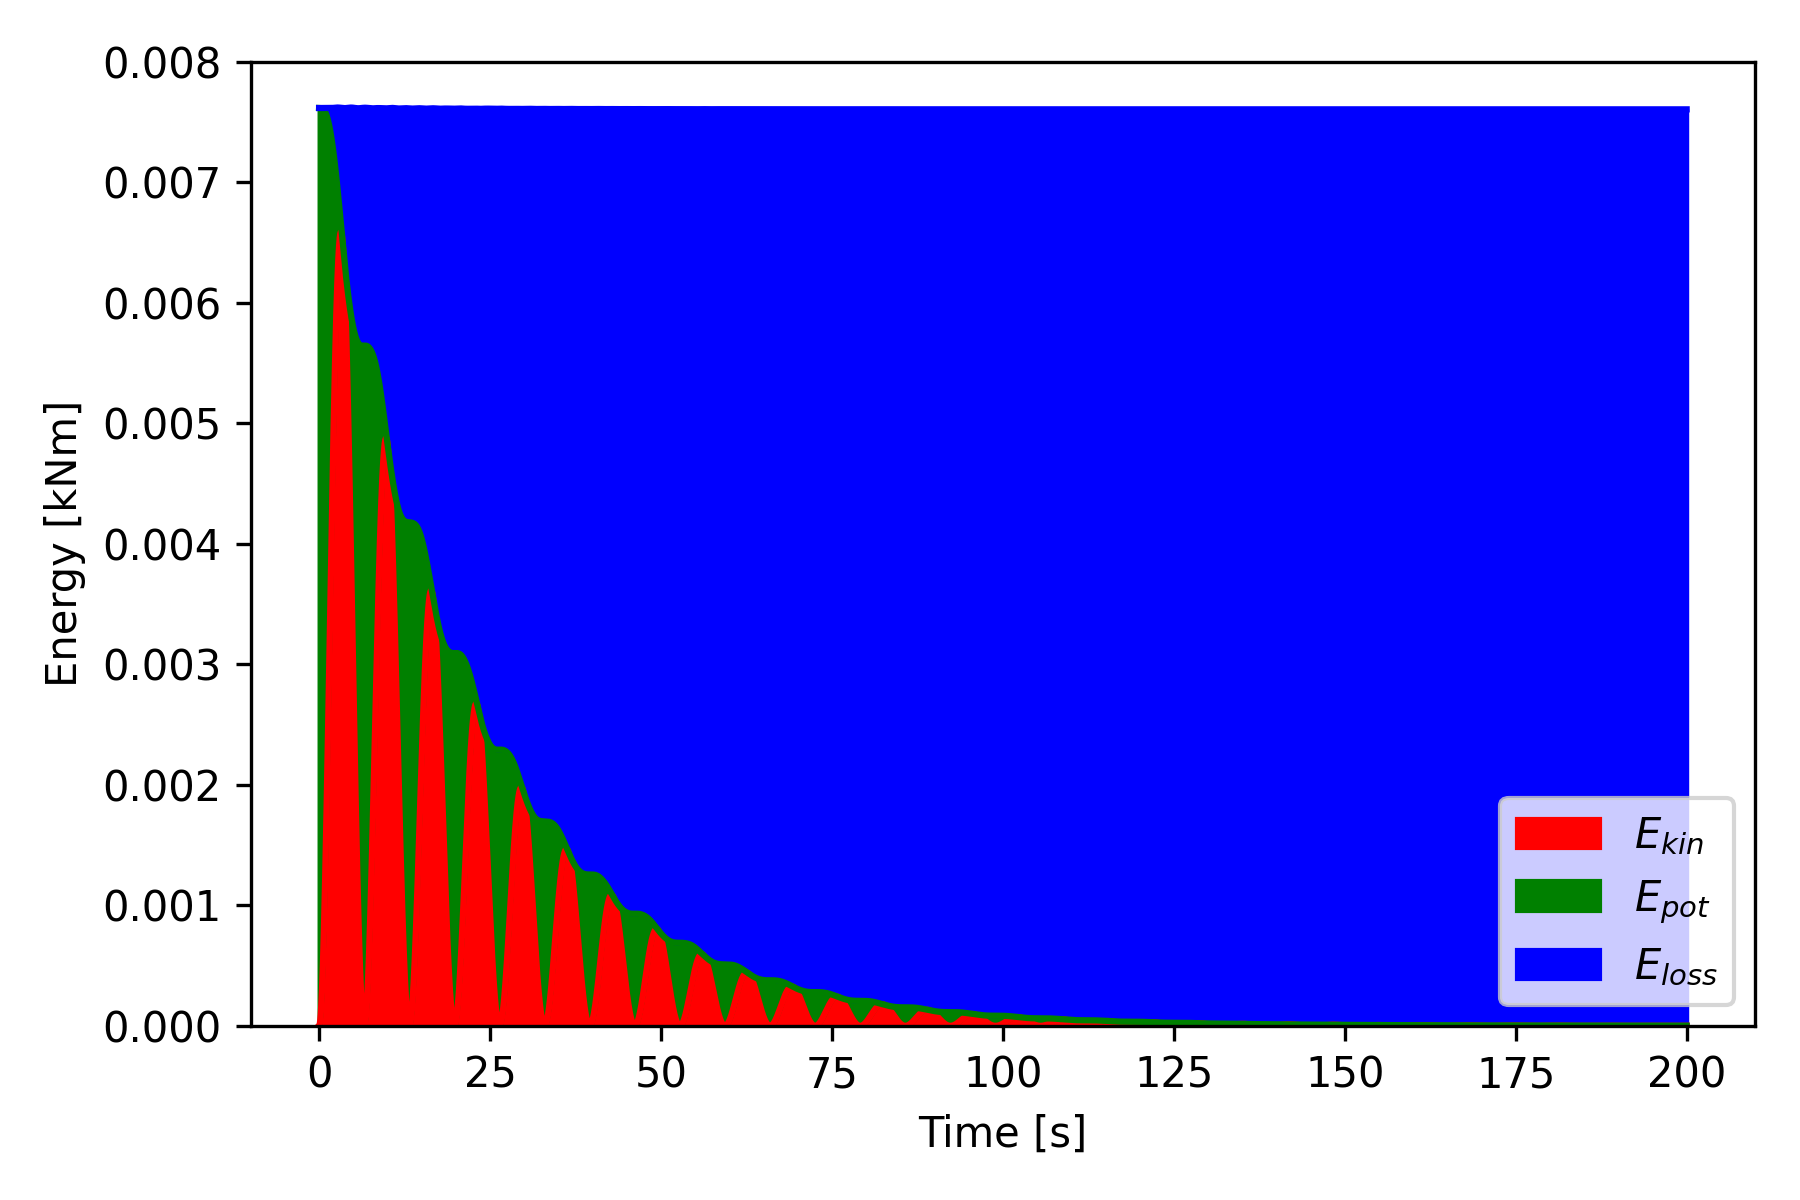
\includegraphics[width = 0.5\textwidth]{figures/energy.png}\end{center}
\vspace{-1cm}
\caption{Energy transfer during roll decay}
\label{fig:energy}
\end{figure}
Time traces of the roll decay roll motion, from model tests as well as
from FNPF and hybrid method simulations are used in this paper to
determine the roll damping. Two different techniques to identify the
damping from these tests are used: the PIT method, described in the next
section and the logarithmic decrement method as described in
\citep{7505983/BYNJ8CFG}.
\subsection*{PIT method to estimate
damping}\label{pit-method-to-estimate-damping}
\label{se:pit}
A parameters identification technique (PIT) similar to
\citep{7505983/EXYJELCU} is used to obtain the damping coefficients from
the roll decay tests. In this technique, parameters in a mathematical
model are determined in order to get the best fit to a roll decay time
signal. A derivation of a mathematical model suitable for this study is
described below together with a description of how the parameters:
damping, stiffness and inertia coefficients are determined. The roll
decay motion can be expressed in general form according to
\citep{7505983/KL7A3RIV} which is the same equation as in
\citep{7505983/FB64RGPF} but with nonlinear stiffness:
\begin{equation}
A_{44} \ddot{\phi} + \operatorname{B_{44}}\left(\dot{\phi}\right) + \operatorname{C_{44}}\left(\phi\right) = 0
\label{eq:roll_decay_equation_general_himeno}
\end{equation}
Where $B_{44}(\dot{\phi})$ and $C_{44}(\phi)$ are the damping and
stiffness models. A quadratic model can be obtained by using cubic
damping \citep{7505983/FB64RGPF}:
\begin{equation}
\operatorname{B_{44}}\left(\dot{\phi}\right) = B_{1} \dot{\phi} + B_{2} \left|{\dot{\phi}}\right| \dot{\phi}
\label{eq:b44_quadratic_equation}
\end{equation}
And a higher order stiffness model \citep{7505983/KL7A3RIV}:
\begin{equation}
\operatorname{C_{44}}\left(\phi\right) = C_{1} \phi + C_{3} \phi^{3} + C_{5} \phi^{5}
\label{eq:restoring_equation_cubic}
\end{equation}
The total equation is then written:
\begin{equation}
A_{44} \ddot{\phi} + \left(B_{1} + B_{2} \left|{\dot{\phi}}\right|\right) \dot{\phi} + \left(C_{1} + C_{3} \phi^{2} + C_{5} \phi^{4}\right) \phi = 0
\label{eq:roll_decay_equation_quadratic}
\end{equation}
This mathematical model can be reduced to a quadratic damping model when
$B_3=0$ and a linear model when $B_2=B_3=0$. This equation does not
have one unique solution however. If all parameters would be multiplied
by a factor $k$ these parameters would also yield as a solution to the
equation. All parameters are therefore divided by the total inertia
$A_{44}$ (including added mass inertia), replacing the parameters with
new helper parameters such as: $B_{1A} = B_1/A_{44}$. The equation is
now rewritten with these new parameters which have unique solutions:
\begin{equation}
\left(B_{1A} + B_{2A} \left|{\dot{\phi}}\right|\right) \dot{\phi} + \left(C_{1A} + C_{3A} \phi^{2} + C_{5A} \phi^{4}\right) \phi + \ddot{\phi} = 0
\label{eq:roll_decay_equation_quadratic_A}
\end{equation}
The parameters of this equation can be identified using least square fit
if the time signals $\phi(t)$, $\dot{\phi}(t)$ and
$\ddot{\phi}(t)$ are all known. This is the case for the results from
the FNPF simulations but not from the model tests, where only the roll
signal $\phi(t)$ is known. The other time derivatives can be estimated
using numerical differentiation of a low-pass filtered roll signal or
Kalman filtered roll signal. The filtering will however introduce some
errors in itself. So instead of using this "Differentiation approach",
it has been found that solving the differential equation numerically for
estimated parameter values determined using optimization similarly to
what was used by \citep{7505983/FJHQJJUH} and \citep{7505983/24TNAV5Z}
gives the best parameter estimation. One problem with this "Integration
approach" is that in order to converge, the optimization needs a
reasonable first guess of the parameters. The Differentiation approach
has therefore been used as a pre-step to obtain a very good first guess
of the parameters that can be passed on to the Integration approach.
This has been used for both signals from FNPF and model tests where in
the latter case numerical differentiation is used.
\quad The differential equation is numerically solved as an initial
value problem, where the initial states for $\phi(t)$,
$\dot{\phi}(t)$ and $\ddot{\phi}(t)$ are used to estimate the
following states, by conducting very small time steps using the
following expression for the acceleration:
\begin{equation}
\ddot{\phi} = - B_{1A} \dot{\phi} - B_{2A} \left|{\dot{\phi}}\right| \dot{\phi} - C_{1A} \phi - C_{3A} \phi^{3} - C_{5A} \phi^{5}
\label{eq:eq_phi1d}
\end{equation}
This numerical solution can be compared with an analytical solution for
a linear model.  For this case the relation between $\zeta$ and $B_1$ can
be expressed as:
\begin{equation}
B_{1} = 2 A_{44} \omega_{0} \zeta
\label{eq:B_1_zeta_eq}
\end{equation}
and the natural frequency can be obtained from:
\begin{equation}
\omega_{0} = \sqrt{\frac{C_{1}}{A_{44}}}
\label{eq:omega0_eq}
\end{equation}
The analytical and numerical solutions are very similar according to the
example: $A_{44} = 1.0$, $B_1 = 0.3$, $C_1 = 5.0$ shown in
Fig.\ref{fig:analytical_numerical}.
\begin{figure}[H]
\begin{center}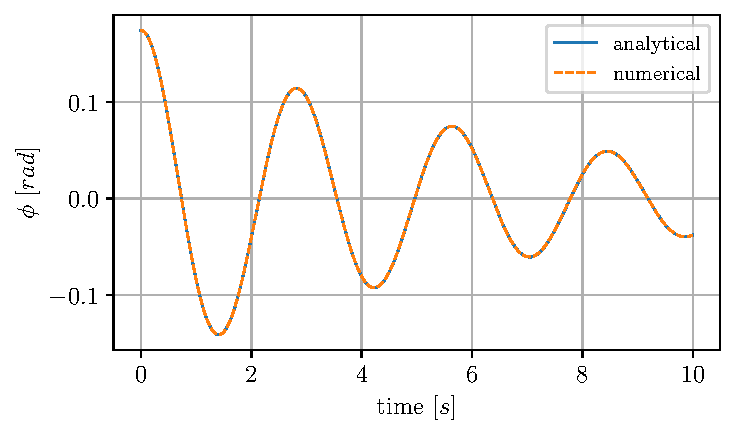
\includegraphics[width = 0.5\textwidth]{figures/analytical_numerical.pdf}\end{center}
\vspace{-1cm}
\caption{Comparison of analytical solution and numerical simulation of a roll decay test.}
\label{fig:analytical_numerical}
\end{figure}

\section{Validation study cases}\label{validation-study-cases}

\label{sec:validation}

    The hybrid method in this paper is investigated using the well known
KVLCC2 test case. This ship was selected partly because it is a well
known test case and also because it does not have any bilge keels.
Ikeda's method contain methods to predict damping from various
components, where the bilge keels is one of them. Results from roll
decay simulations made with the hybrid method will be compared to
corresponding model test data from the SSPA Maritime Dynamics
Laboratory. From these model tests, only the total damping can be
observed. Reducing the number of components by having no bilge keels
will therefore give more insight into the remaining components.
 
            
    
    
\begin{table}[H]
\\scriptsize
\center
\caption{KVLCC2 model data}
\label{tab:kvlcc2_model_data}
\begin{tabular}{llllllll}
\toprule\addlinespace
$L_{pp}$ & $beam$ & $v_{cg}$ & $k_{xx}$ & $S$ & $V$ & $rho$ & $T$\\ 
\midrule$[m]$ & $[m]$ & $[m]$ & $[m]$ & $[m^2]$ & $\left[\frac{m}{s}\right]$ & $\left[\frac{kg}{m^3}\right]$ & $[m]$\\ 
4.706 & 0.853 & 0.274 & 0.341 & 5.981 & 0.993 & 1000.0 & 0.3059\\ 

\bottomrule
\end{tabular}
\end{table}

    
 
            
    
    \begin{figure}[H]
        \begin{center}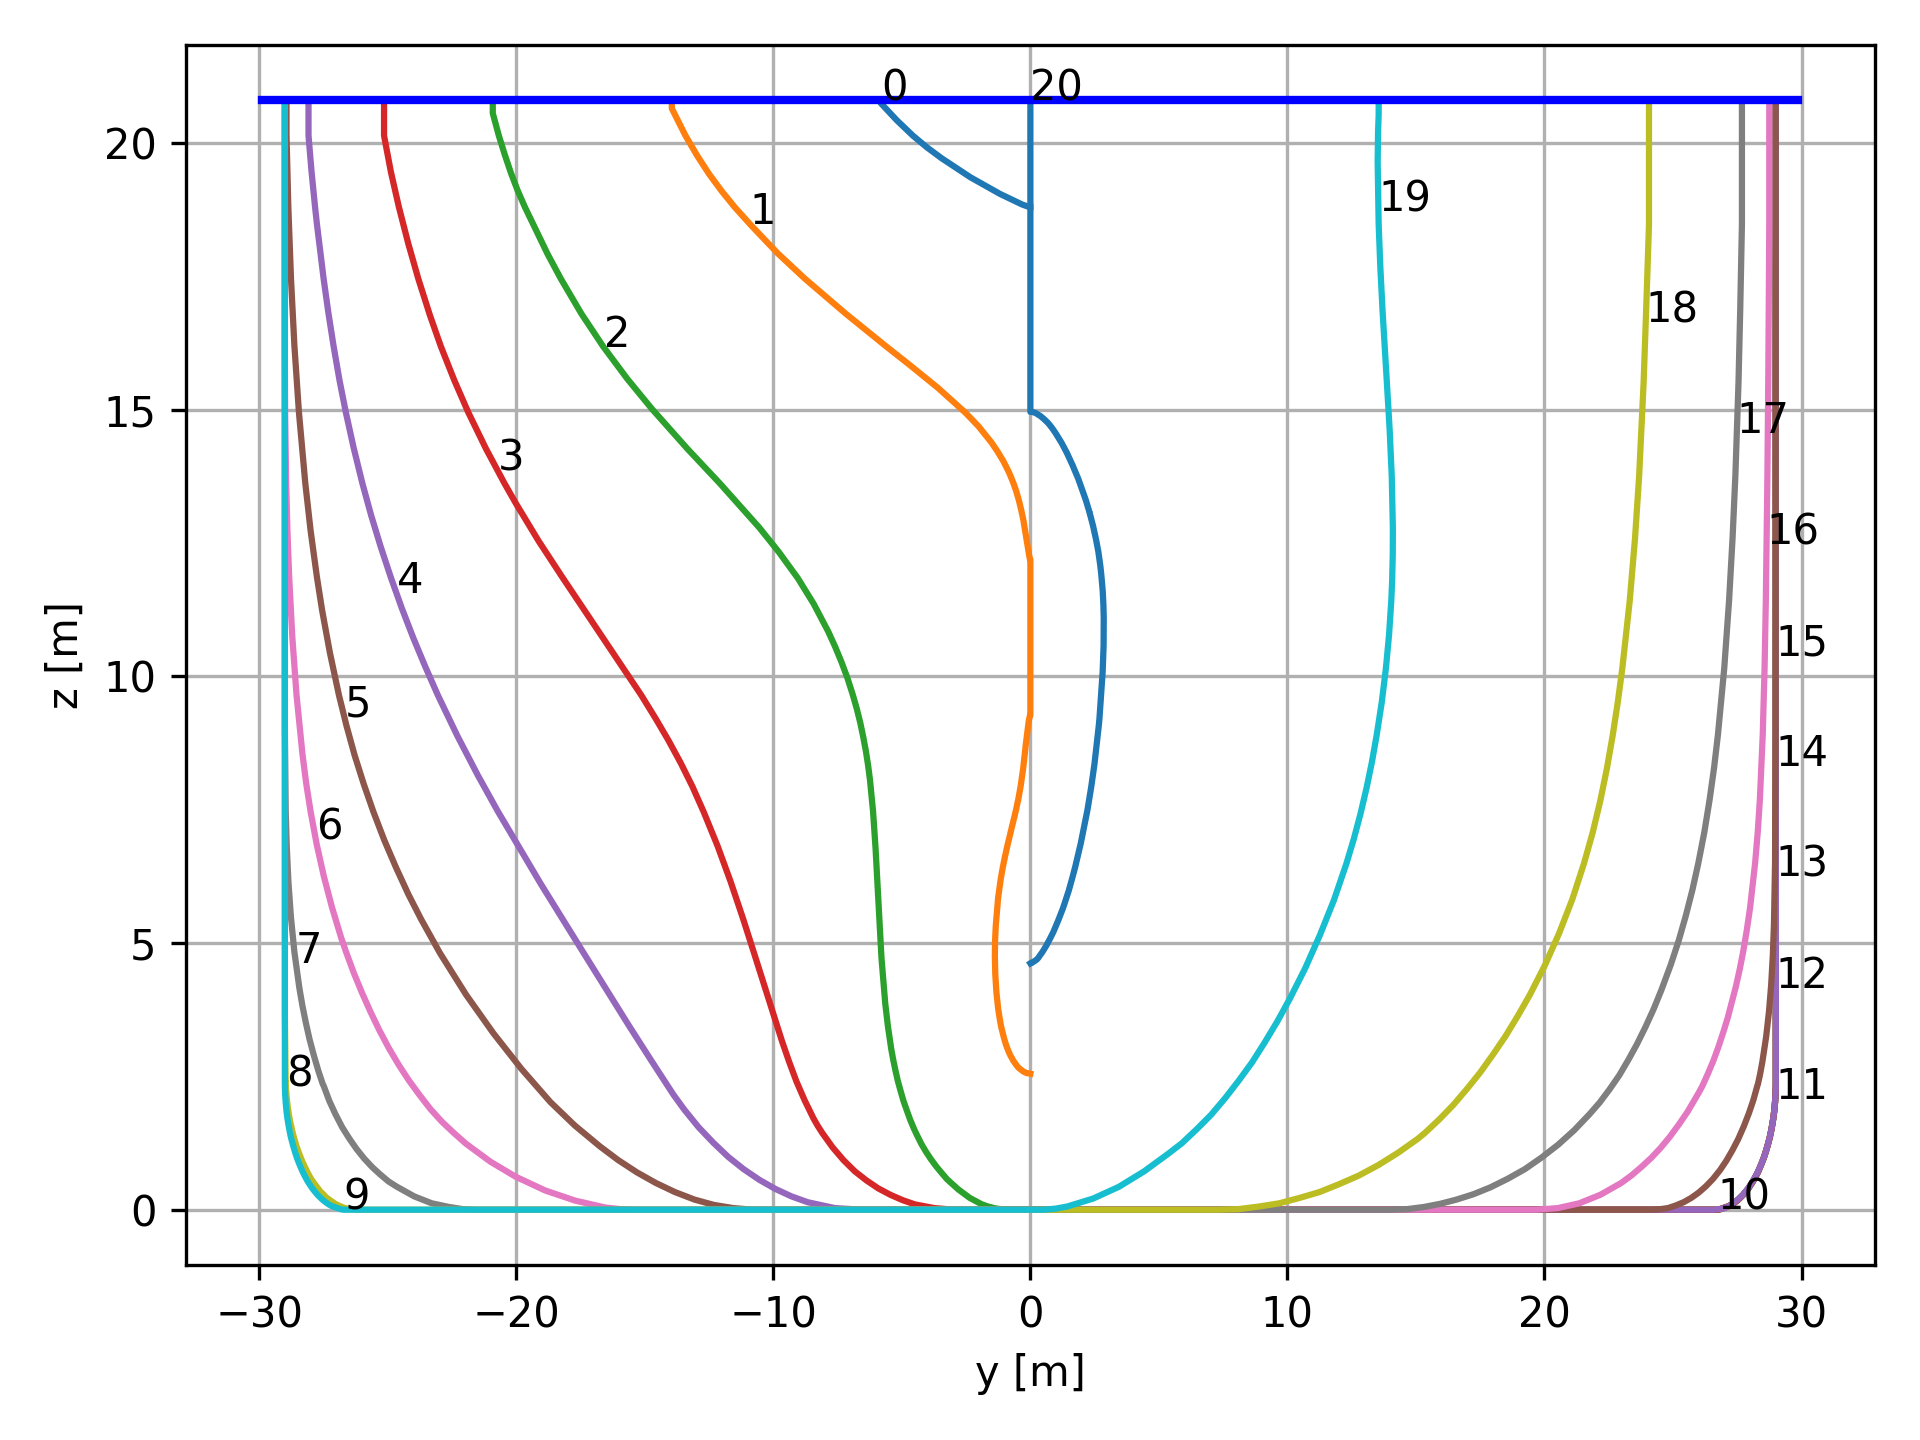
\includegraphics[width = 0.5\textwidth]{figures/body_plan.png}\end{center}
        \vspace{-1cm}
        \caption{Body plan}
        \label{fig:body_plan}
    \end{figure}
    

    
\section{Results}\label{results}

    \subsection{Roll decay model tests}\label{roll-decay-model-tests}

\subsubsection{0 knots}\label{knots}

Data from two roll decay model tests conducted at zero speed were
available:
\href{../../notebooks/01.2_select_suitable_MDL_test_KLVCC2.ipynb\#rolldecay}{Roll
decay model tests 0 knots}. These tests where analyzed by fitting a
\href{../../notebooks/01.2_select_suitable_MDL_test_KLVCC2.ipynb\#cubic_model}{Cubic
model} to the model test data. The two models were very similar in terms
of roll damping and stiffness, suggesting good repeatability in the
model tests as well as in the parameter identification technique (PIT)
used. The individual damping from each oscillation obtained with the
logarithmic decrement method are very scattered, but this does not seem
to influence the two models for the 0 speed case, which are very
similiar.

    \subsubsection{15.5 knots}\label{knots}

Data from one roll decay model tests conducted at a ship speed
corresponding to 15.5 knots full scale ship speed was also available.
This model tests was analyzed in the same way as the other tests. It was
found that the damping was higher at speed. The ship got a small
\href{../../notebooks/01.3_select_suitable_MDL_test_KLVCC2_speed.ipynb\#yawrate}{yaw
rate} at the end of test, giving a small steady roll angle due to the
centrifugal force. Since this effect is not included in the matematical
model used, the steady roll angle was instead removed by removing the
linear trend in the roll angle signal.

    \begin{center}
    \adjustimage{max size={0.9\linewidth}{0.9\paperheight}}{output_89_0.pdf}
    \end{center}
    { \hspace*{\fill} \\}
    
    \subsection{Ikeda's method}\label{ikedas-method}

    When looking at predictions for KVLCC2 at 0 speed made with regular
Ikeda's method, it was found that the eddy damping \(B_E\) was too high
compared with the regular implementation, compared to the model test
results. Eventhough the rest of the components would also be
overpredicted, the \(B_E\) would still be too large. The eddy damping
calculated with \(C_r\) predicted with the descision tree gave much
better agreement.

    \begin{center}
    \adjustimage{max size={0.9\linewidth}{0.9\paperheight}}{output_93_0.pdf}
    \end{center}
    { \hspace*{\fill} \\}
    
    \subsection{FNPF}\label{fnpf}

Simulations of roll decay tests were conducted with FNPF for each model
test. The results from these simulations can be seen in the figure
below.

    \begin{center}
    \adjustimage{max size={0.9\linewidth}{0.9\paperheight}}{output_96_0.pdf}
    \end{center}
    { \hspace*{\fill} \\}
    
    \subsection{Roll damping prediction with Hybrid
method}\label{roll-damping-prediction-with-hybrid-method}
Replacing the wave damping $B_W$, for the zero speed case above, with values obtained with FNPF is shown below. 
    \begin{center}
    \adjustimage{max size={0.9\linewidth}{0.9\paperheight}}{output_99_0.pdf}
    \end{center}
    { \hspace*{\fill} \\}
    
    FNPF gave stable results at zero speed, but very unstable results at
speed, due to what was thought to be memory effects. For the speed case
the viscous damping was instead present during the actual FNPF
simulations. The viscous damping was included by adding a linear
\(B_{visc,1}\) and quadratic \(B_{visc,2}\) damping term the equation of
motions in the FNPF. The results are compared with corresponding results
from the model tests.

    \begin{center}
    \adjustimage{max size={0.9\linewidth}{0.9\paperheight}}{output_101_0.pdf}
    \end{center}
    { \hspace*{\fill} \\}
    
    The results using the Hybrid method for Run 3 at speed gives very
similar results to the corresponding model tests.

    \begin{center}
    \adjustimage{max size={0.9\linewidth}{0.9\paperheight}}{output_103_0.pdf}
    \end{center}
    { \hspace*{\fill} \\}
    
    The coefficients obtained from model tests, FNPF and Hybrid method are
summarized in model scale units in the table below:
 
            
    
    \begin{longtable}[c]{@{}lllllll@{}}
\toprule\addlinespace
run & method & $F_n$ & $\omega_0$ & $B_1$ & $B_2$ & $B_3$\\\addlinespace 
\midrule\endhead
1 & model test & 0.0 & 2.461405663797153 & 2.960431148229692 & -6.520487128705247 & 43.7753590783464\\\addlinespace 
2 & model test & 0.0 & 2.461149414341689 & 2.879736279200558 & -5.874151219904037 & 41.50366418695269\\\addlinespace 
2 & FNPF & 0.0 & 2.469512621237472 & 0.14245882294522433 & 2.9442349635220273 & 0.0\\\addlinespace 
3 & model test & 0.14231828016230666 & 2.4675051791344322 & 7.523313711481077 & 7.0280627607638 & 0.3897887036233833\\\addlinespace 
3 & FNPF & 0.14231828016230666 & 2.4731115844417735 & 1.939382895537425 & 2.876088787299491 & 0.0\\\addlinespace 
3 & FNPF & 0.14231828016230666 & 2.4672709863288573 & 1.8288702419438334 & 3.3099823707085987 & 0.0\\\addlinespace 
3 & FNPF & 0.14231828016230666 & 2.4531795386475976 & 2.503610883554999 & 1.3308576126192526 & 0.0\\\addlinespace 
3 & FNPF & 0.14231828016230666 & 2.4642154500169404 & 7.612597393349741 & 8.176912123526904 & 0.0\\\addlinespace 
3 & FNPF & 0.14231828016230666 & 2.440717566554755 & 7.8985005775656605 & 4.593428224531338 & 0.0\\\addlinespace 
\bottomrule 
 \end{longtable}

    

    
\section{Conclusions}\label{conclusions}

    


%\input{references}
% Chose bibliography style
%\bibliographystyle{plainnat}
\bibliographystyle{apalike}
\bibliography{references}


\appendix
\section{Appendix}\label{appendix}

    \subsection{Lewis sections}\label{lewis-sections}

    The Lewis section coefficients were calculated as:
 
            
    
    \begin{equation}
D_{1} = \frac{4 \sigma}{\pi} + \frac{\left(H_{0} - 1\right)^{2} \left(- \frac{4 \sigma}{\pi} + 1\right)}{\left(H_{0} + 1\right)^{2}} + 3
\label{eq:equation}
\end{equation}

    
 
            
    
    \begin{equation}
a_{3} = \frac{- D_{1} + \sqrt{9 - 2 D_{1}} + 3}{D_{1}}
\label{eq:equation}
\end{equation}

    
 
            
    
    \begin{equation}
a_{1} = \frac{\left(H_{0} - 1\right) \left(a_{3} + 1\right)}{H_{0} + 1}
\label{eq:equation}
\end{equation}

    

    \subsection{KVLCC2}\label{kvlcc2}
 
            
    
    
\begin{table}[H]
\\scriptsize
\center
\caption{KVLCC2 section table}
\label{tab:kvlcc2_section_table}
\begin{tabular}{llllllll}
\toprule\addlinespace
$x$ & $beam$ & $T_s$ & $\sigma$ & $\frac{OG}{d}$ & $R_b$ & $a_1$ & $a_3$\\ 
\midrule$[m]$ & $[m]$ & $[m]$ & $[-]$ & $[-] & $[m]$ & $[-]$ & $[-]$\\ 
-0.0808 & 0.1712 & 0.0294 & 0.594 & 1.1 & 0.0976 & 0.5341 & 0.0935\\ 
0.1494 & 0.4102 & 0.2684 & 0.2433 & 0.1205 & 0.623 & -0.1824 & 0.3651\\ 
0.4125 & 0.6151 & 0.3059 & 0.4922 & 0.1058 & 0.6672 & 0.0032 & 0.1916\\ 
0.6427 & 0.7394 & 0.3059 & 0.6537 & 0.1058 & 0.6041 & 0.1024 & 0.0836\\ 
0.9058 & 0.8259 & 0.3059 & 0.7858 & 0.1058 & 0.5021 & 0.1489 & -0.0002\\ 
1.1361 & 0.851 & 0.3059 & 0.878 & 0.1058 & 0.3847 & 0.1542 & -0.0576\\ 
1.3663 & 0.8529 & 0.3059 & 0.9445 & 0.1058 & 0.2596 & 0.1482 & -0.0998\\ 
1.6294 & 0.8529 & 0.3059 & 0.9838 & 0.1058 & 0.1404 & 0.144 & -0.1255\\ 
1.8596 & 0.8529 & 0.3059 & 0.9974 & 0.1058 & 0.0566 & 0.1425 & -0.1345\\ 
2.1227 & 0.8529 & 0.3059 & 0.998 & 0.1058 & 0.0499 & 0.1424 & -0.1349\\ 
2.3529 & 0.8529 & 0.3059 & 0.998 & 0.1058 & 0.0499 & 0.1424 & -0.1349\\ 
2.5866 & 0.8529 & 0.3059 & 0.998 & 0.1058 & 0.0499 & 0.1424 & -0.1349\\ 
2.8537 & 0.8529 & 0.3059 & 0.998 & 0.1058 & 0.0499 & 0.1424 & -0.1349\\ 
3.0874 & 0.8529 & 0.3059 & 0.998 & 0.1058 & 0.0499 & 0.1424 & -0.1349\\ 
3.3211 & 0.8529 & 0.3059 & 0.9979 & 0.1058 & 0.0501 & 0.1424 & -0.1349\\ 
3.5882 & 0.8528 & 0.3059 & 0.9912 & 0.1058 & 0.1032 & 0.1431 & -0.1304\\ 
3.8219 & 0.8454 & 0.3059 & 0.9701 & 0.1058 & 0.1898 & 0.1416 & -0.1166\\ 
4.0556 & 0.8141 & 0.3059 & 0.9358 & 0.1058 & 0.273 & 0.1285 & -0.0949\\ 
4.2893 & 0.7078 & 0.3059 & 0.8981 & 0.1058 & 0.3206 & 0.0676 & -0.0718\\ 
4.5564 & 0.4148 & 0.3059 & 0.8566 & 0.1058 & 0.2911 & -0.1835 & -0.0438\\ 
4.7901 & 0.084 & 0.2379 & 0.4708 & 0.136 & 0.222 & -0.7722 & 0.103\\ 

\bottomrule
\end{tabular}
\end{table}

    


    % Add a bibliography block to the postdoc
    
    
    


\end{document}
